%----------------- CHAPTER 3 -------------------------------------------
%------ Length Sensing and Control -----------------------------------
%% 
%% Describes the signal extraction for the length DOFs
%% 
%% also the coupling of noise sources on the light
%% 
\chapter{Signal Extraction}
\label{chap:signals}

\begin{figure}[!h]
\centerline{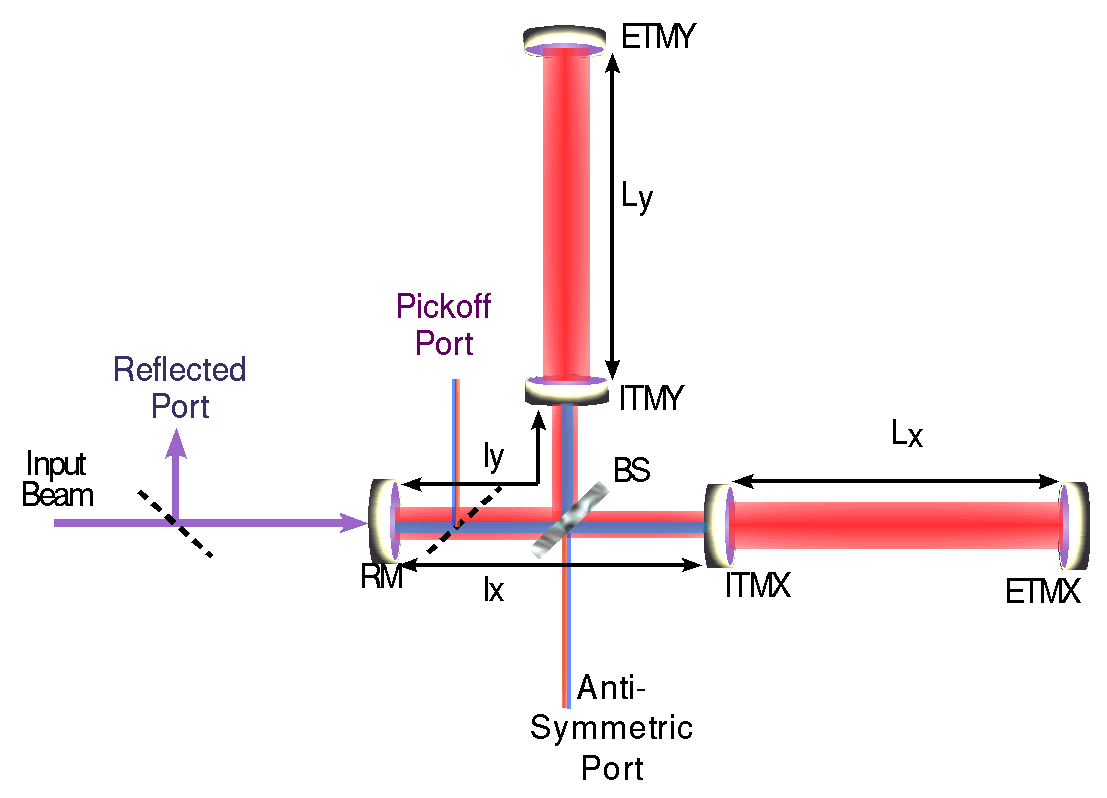
\includegraphics[angle=0,width=6.5in]{Figures/Chap3/IFO2.png}}
\end{figure}
\clearpage

In order to achieve the strain sensitivity goal, multiple resonant cavities
are used to store the light in the interferometer. To keep the cavities
on resonance an active feedback system is employed. This chapter will 
describe how the cavity lengths are sensed and controlled.

\begin{figure}[!h]
\centerline{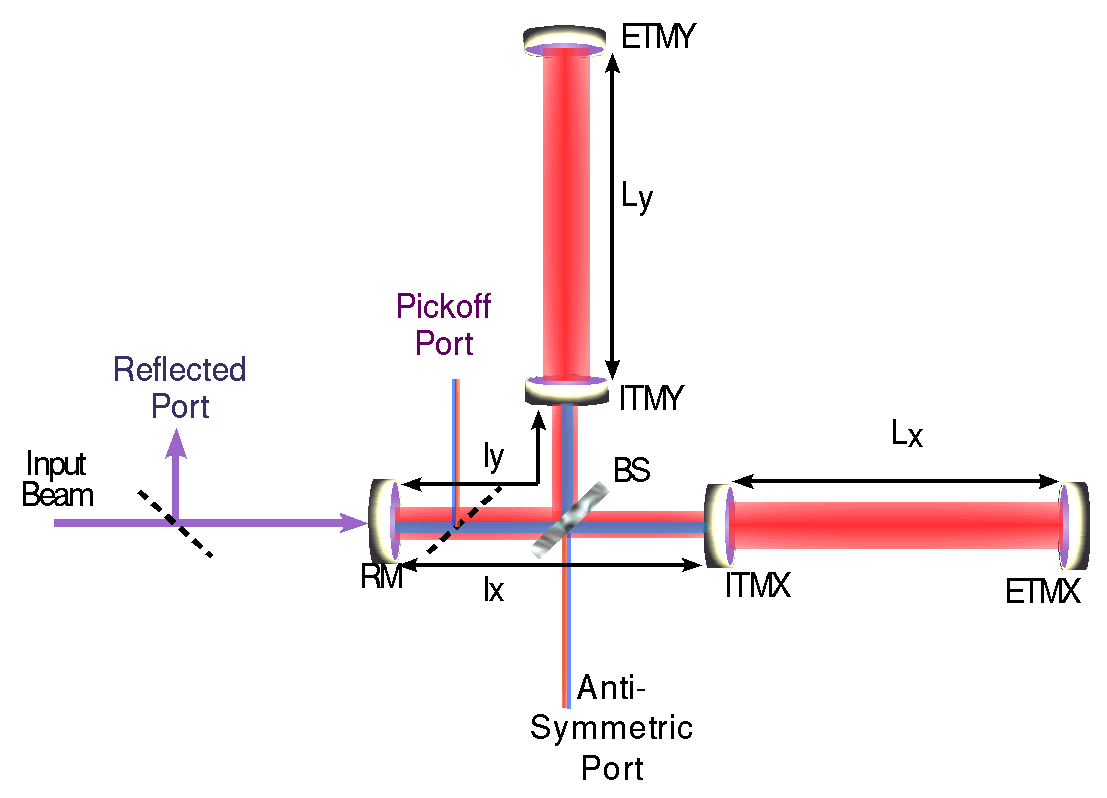
\includegraphics[angle=0,width=6.5in]{Figures/Chap3/IFO2.png}}
\caption[Length Definitions]{Designations of length degrees-of-freedom and signal
                  readout ports. Further details in Appendix~\ref{app:variables}}
\label{fig:DOFs}
\end{figure}



%- - - - - - - - - -  -  -  - - - - - - -  -  -  -   -   -    -    -     -      -
%- - -  SIGNAL READOUT - - - - - - -  -  -  -   -   -    -    -     -      -
%- - - - - - - - - -  -  -  - - - - - - -  -  -  -   -   -    -    -     -      -
\section{Signal Readout Scheme}

The steady state signal readout problem is this: to find the functions that
relate the change of a length with optical signals at the readout ports. 
This solutions is a sensing matrix of the form

\begin{equation}
\vec{V} = \overleftrightarrow{S} \otimes \vec{X}
\end{equation}
where $\vec{V}$ is the vector of voltage readouts, $\vec{X}$ is the vector of
mirror motions, and $\overleftrightarrow{S}$ is the sensing matrix. Each 
element of $\overleftrightarrow{S}$ can be frequency dependent. 

Previous works \cite{Regehr:Thesis,Sigg:FreqResp} have calculated 
this matrix. This section and the rest of the thesis will use the more modern 
notation of \cite{Sigg:FreqResp}. \textbf{Appendix~\ref{app:variables} includes 
the definitions of variables used in the following formulas}.

The physical detector used in the sensing scheme is a photodiode. Since this
detector is only sensitive to power and not the electric field directly, the
trick in the readout is to produce power fluctuations on the readout ports.

To make the measurements at a frequency at which the technical laser noise is
small, the beam incident on the interferometer is phase modulated at 
an angular (radio) frequency, $\omega_m \approx 2 \pi \times$25 MHz. The resulting 
electric field is:

\begin{equation} 
  \begin{aligned} \label{eq:InputBeam}
  E_{in} &= E_0 e^{i \Gamma cos(\omega_m t)} \\
         &\simeq E_0 \left \{ J_0(\Gamma) 
                    + i J_1(\Gamma)e^{+i \, \omega_m t}
                    + i J_1(\Gamma)e^{-i \, \omega_m t}
                    - J_2(\Gamma) e^{+i \, 2 \omega_m t}
                    - J_2(\Gamma) e^{-i \, 2 \omega_m t}
                     \right \}
  \end{aligned}  
\end{equation}
where $\Gamma$ is the modulation depth in radians, $\omega_m$ is the 
modulation angular frequency, $J_n$ is the n$^{\mbox{\tiny th}}$ order Bessel
function of the first kind, and $E_0$ is the unmodulated field of the laser. In
the LIGO interferometers, $\Gamma \approx 0.4$.

The first order Radio Frequency (RF) sidebands and carrier field can be treated
as three fields, each at different frequencies. Each field will have different
reflection and transmission coefficients at each point within the complex coupled 
cavity system of the interferometer. The signal 
readout scheme used in LIGO takes advantage of this dispersion. The scheme is a 
variant of a (now standard) RF reflection locking
technique~\cite{Pound:Locking,Drever:PDH}. To implement this, the 
RF photodetector signal at each port is demodulated at the modulation frequency
used to drive the Pockels cell. The In-phase (cosine) and Quadrature-phase
(sine) components are then separately recorded and/or used in the feedback
control (see Chapter~\ref{chap:controls}).

The naming convention for the interferometer lengths is described in
Appendix~\ref{app:variables}. For the output signals the convention is:
(Port)\_Quadrature. So for example the POB\_Q signal is the quadrature
phase of the demodulated signal from the recycling cavity Pick-Off of the
Beamsplitter. The REFL
signals refer to the signals taken from the light reflected back to the
symmetric port from the interferometer and the AS signals are from the 
Anti-Symmetric port.

As is the convention in \cite{Regehr:Thesis} and \cite{Sigg:FreqResp}, all of
these signal formulae are only valid for frequencies below the arm cavity
free spectral range ($\sim$37.5 kHz for a 4 km cavity). The expressions were
derived using the 'audio sideband' approach: a mirror moving at a frequency,
$f_a$, impresses phase modulation sidebands on the reflected field 
at +/- $f_a$ relative to the incident field. So an incident field with three
frequency components will be reflected with nine frequencies.

Effects from higher order spatial modes are not included here.


%- - - - - - - - - -  -  -  - - - - - - -  -  -  -   -   -    -    -     -      -
%- - - MATRIX ELEMENTS - - - - - - -  -  -  -   -   -    -    -     -      -
%- - - - - - - - - -  -  -  - - - - - - -  -  -  -   -   -    -    -     -      -
\section{Elements of the Sensing Matrix}

\begin{figure}[!h]
\centerline{
\includegraphics[angle=0,width=6.0in]{Figures/Chap3/plant.pdf}}
\caption[LLO Optical Plant]{Plotted are the signal strengths for the L1 interferometer
                in Watts at the modulation frequency per micron of optic
                motion. The solid lines are the diagonal plant elements
                used for the interferometers main length loops. The dashed
                lines are off-diagonal elements. A pickoff fraction of
                80 ppm has been used to calculate the POB signals. All curves are
                for the $\sim$1.6 W of input power in L1 during the S2 run.}
\label{fig:Plant}
\end{figure}
The control system (Chapter~\ref{chap:controls}) adjusts the arm lengths to 
produce a dark fringe
for the carrier. Since the Michelson arm lengths are not equal, dark for the
carrier field does not necessarily mean dark for the sidebands. This arm
length asymmetry ($l_- \approx$ 17 cm) has been designed to transmit a few percent 
of the sideband power from the recycling cavity to the AS port.

Signals at the AS port come from the carrier field beating against the 
static sideband field. Differential changes in the arm cavity lengths ($L_{-}$) 
or in the Michelson length ($l_{-}$) cause a first order differential
phase shift in the carrier fields returning to the beamsplitter from each arm.

\begin{equation}
[ L_{-} \rightsquigarrow AS\_Q ] = -\aleph \, g_{cr} t_{sb} r_{c}'
                          \frac{1}{1 + i f / f_c}
                          k \, \delta L_{-}
\label{eq:darm2asq}
\end{equation}
The notation of the L.H.S. of Equation~\ref{eq:darm2asq}, and all of the following
equations representing elements of the sensing matrix, denotes a transfer
function from one degree of freedom to one readout signal.

Changes occurring faster than the storage time of
the arm cavities do not experience the full buildup of the cavity and are
attenuated compared to low frequencies. Gravitational wave strain signals are read 
out through this same mechanism and so are similarly attenuated at high frequencies.


\begin{equation}
[ l_{-} \rightsquigarrow  AS\_Q ] = \aleph \, g_{cr} t_{sb} r_{c} 
                          \frac{1}{1 + i f / f_c}
                          k \, \delta l_{-}
\label{eq:mich2asq}
\end{equation}
Changes in the Michelson length also show up in this signal but down by a factor of
$r_{c}'/r_{c}$ (which is $\sim 140$ for the LIGO interferometers). This factor is
the 'phase gain' or build-up factor of the arm cavities. Fluctuations above the
arm cavity pole are not resonant in the arm cavities. Since the arms are over-coupled
cavities, the sign of the reflected field changes depending on whether the
incident field is resonant or not. So the high frequencies get a sign flip and
fall out of resonance in the recycling cavity.


The field reflected from the interferometer contains signals contributed by 
both the sidebands and the carrier since both are resonant in parts of the interferometer.

\begin{equation}
[ L_{+} \rightsquigarrow  REFL\_I ] = 2 \aleph \, g_{cr}^{2} r_{sb} r_{c}'
                            \frac{1}{1 + i f / f_{cc}}
                            k \, \delta L_{+}
\label{eq:carm2refli}
\end{equation}
Common mode changes of the arm lengths affect only the carrier field since the sidebands
are not resonant in the arms. This signal has 2 factors of $g_{cr}$ in it; one, 
since the carrier field in the arms is amplified by the recycling cavity and 
another, because the common arm signal is resonant in the recycling cavity. 
At the reflected port, these carrier audio sidebands beat against the static 
RF sidebands.


\begin{equation}
[ l_{+} \rightsquigarrow  REFL\_I ] = 2 \, \aleph \, \left [ g_{sb}^{2} r_{cr} r_{M}  
                            + g_{cr}^{2} r_{sb} r_{c} 
                            \frac{1}{1 + i f / f_{cc}} \right ]
                            k \, \delta l_{+}
\label{eq:prc2refli}
\end{equation}
The REFL\_I signal produced by a change of the power recycling cavity average length 
($l_{+}$) is more complicated. Since both the sidebands and carrier are resonant in 
the recycling cavity, both are modulated by the $l_+$ length change. The carrier 
component is filtered above $\sim$1 Hz by the coupled cavity resonance and so the main 
contribution above 100 Hz is from the RF sidebands' audio sidebands beating 
with the static carrier.


\begin{equation}
[l_{-} \rightsquigarrow  REFL\_Q ] = - \aleph \, g_{sb} t_{sb} r_{cr} k \, \delta l_{-}
\label{eq:mich2reflq}
\end{equation}
The quadrature phase signals at the REFL and PO ports are produced in a
different way. Changes in the Michelson length change produce differential changes
in the sideband fields reflected from the Michelson back towards the RM. At the
reflected port, the difference between the amplitudes of the upper and lower
sidebands produce a signal 90 degrees out of phase with the REFL\_I signal. In
a symmetric arm length Michelson interferometer, there would be no Q-phase
signal, since the reflectivity for the sidebands would be a quadratic
function of $l_{-}$.



\begin{equation}
[ L_{+} \rightsquigarrow  POB\_I ] = -2 \aleph \, \frac{g_{cr}^{2} g_{sb}}{t_{RM}} r_{M} r_{c}'  
                  \frac{1}{1 + i f / f_{cc}} k \, \delta L_{+}
\label{eq:carm2pobi}
\end{equation}
The signal from the pick off inside the recycling cavity is very similar to the
one in reflection. The main difference being that it does not depend delicately
on the coupling of the sideband to the recycling cavity, but instead is produced
by beating the carrier audio sidebands against the resonant sideband field.


\begin{equation}
[ l_{+} \rightsquigarrow  POB\_I ] = 2 \aleph \, \frac{g_{cr} g_{sb}}{t_{RM}} r_{M} r_{c}  
                  \left[g_{cr} \frac{1}{1+i\frac{f}{f_{cc}}} -g_{sb}\right]
                  k \, \delta l_{+}
\label{eq:prc2pobi}
\end{equation}
Very similar to the $[l_{+} \rightsquigarrow REFL\_I]$ element. The main difference
is that the local oscillator field is the carrier field inside the recycling cavity
instead of the carrier reflected from the interferometer.

\begin{equation}
[ l_{-} \rightsquigarrow  POB\_Q ] = -\aleph \, \frac{g_{cr} g_{sb}^2}{t_{RM}} t_{M} 
                                      k \, \delta l_{-}
\label{eq:mich2pobq}
\end{equation}
This element also appears to be similar to the REFL port element but there are two
important differences. First, the signal is independent of the sign of the
carrier coupling since it uses the internal recycling cavity field. Second, the
dominant carrier field in reflection can be the non-modematched component. This
will produce a spurious signal through beating with non-modematched sideband
field.

Since each readout signal is sensitive to multiple degrees of freedom there is some
choice to be made in selecting a particular configuration.
It is fairly clear from these equations and Figure~\ref{fig:Plant} that only AS\_Q 
may be used for reading out the differential arm length. This leaves some other 
combination of the Q-phase signals to read out $l_{-}$. In the absence of 
beam distortions, we would be free to choose whichever combination of the two
gives the best SNR. In the case of the $l_-$ readout, we use the POB\_Q signal
to avoid the junk signal from the mode-mismatch of the carrier and sidebands.

The case for the common mode signals is a little less clear, since in both REFL\_I 
and POB\_I the $L_{+}$ signal is totally dominating the weak $l_{+}$ signal. In a 
perfectly stable, noiseless interferometer
one could take this 2 $\times$ 2 signal matrix and invert it properly to
obtain linearly independent readouts of both degrees of freedom. 

In the real world, this is problematic for two reasons: first, the small fraction of 
light  from the internal recycling cavity pickoff is
so small ($\sim$100 ppm) that the signal-to-noise ratio is much poorer than
the reflected port where all of the light is available and second, even if
the noise were not an issue, this matrix inversion would require subtracting two 
large signals
to produce a very small signal (the $l_+$ signal) and would be overly sensitive
to variations in the optical gain at the REFL and POB ports. To avoid these
issues, the REFL\_I signal is fed back to the laser frequency with a high gain, 
high bandwidth loop (see Section~\ref{sec:CMservo}), effectively driving the 
REFL\_I signal 
to zero. Solving for the newly flattened plant by setting $\mbox{REFL\_I} = 0$, 
gives a new solution for POB\_I which is only sensitive to $l_{+}$:

\begin{equation}
[ l_{+} \rightsquigarrow  POB\_I ] = - 2 \aleph \, \frac{g_{sb}^2 r_M}{t_{RM}r_{sb}}
                           \left [ g_{cr} r_{sb} r_c + g_{sb} r_{cr} r_M \right ]
                           k \, \delta l_{+}
\end{equation}


%- - - - - - - - - -  -  -  - - - - - - -  -  -  -   -   -    -    -     -      -
%- - - DARK PORT SIGNALS - - - - - - -  -  -  -   -   -    -    -     -      -
%- - - - - - - - - -  -  -  - - - - - - -  -  -  -   -   -    -    -     -      -
\section{Dark Port Signal Generation}
\label{sec:darksignals}

Equation~\ref{eq:darm2asq} only deals with the Q phase signal which we use for
the gravitational wave signal readout and the differential arm length control.
It was assumed that the only carrier field at this port comes from the differential
arm length offset. However, a carrier field may also exist in the other phase.
In principle, this should not produce a signal unless there is a corresponding
sideband field in the ``wrong`` phase. Including fields in both phases we get:

\begin{equation}
 \begin{split}
  \frac{E_{AS}}{E_{0}} =& J_{0}(\Gamma) g_{cr} \left [ \frac{\delta r_c}{2} 
                                         + i r_{c}' k \Delta L_- \right ] \\
 \times & J_{1}(\Gamma) t_{M} \left [ \frac{\delta g_{sb}}{2} \cos{\omega_{m} t}
                           + i 2 g_{sb} \sin{\omega_{m} t} \right ]
 \end{split}
\end{equation}
where we have included two asymmetries: $\delta r_c$ is the difference in the
arm cavities' resonant reflectivities for the carrier and $\delta g_{sb}$ is
the difference in the recycling gain between the upper and lower 
first order RF sidebands.

The AS\_Q signal is produced by the beat between the imaginary part of the
carrier field and the imaginary part of the sideband field. The AS\_I signal
is produced by the real components and only exists in the presence of the
two asymmetries.
\begin{equation}
S_{\mbox{\tiny AS\_I}} = \frac{1}{8} \aleph \, g_{cr} t_{M} 
                         \, \delta r_c \, \delta g_{sb}
\label{eq:ASI}
\end{equation}
